\subsubsection{Testing Suite}\label{subsubsec:testing-suite}
Table 3 below covers what software functions and components of the Nav were verified, how they were verified, and
whether each one passed.
Localization estimates are left untested until integration with the Visual Processing Software Subsystem since they
require both subsystems to work together.
\begin{center}
    \begin{tabular}{ |c|c|c|c| }
        Name & Objectives & Definition & Results \\
        A* & Correctness - Is the algorithm implemented in a sound manner? & Unit tests & Pass \\
        Nav & Safety - Does it avoid steep (>20° incline) slopes? Adherence to the supplied parameters - Start and end position and orientation, minimum turn radius Length - Does it take a reasonable path, not looping or backtracking? & Unit tests & Pass \\
        Mesh to Grid & Faithfulness - Does the grid representation closely match the physical terrain? & Human-reviewed & Pass
    \end{tabular}
\end{center}
\subsubsection{Changes from Previous Verification Plan}\label{subsubsec:changes-to-plan}
Previously, the gradient grid obtained from the triangle mesh did not accurately reflect the physical environment in
some cases.
The biggest issue was that overhangs with vertical faces, when flattened to 2D, appeared as a massive spike in the
terrain heightmap.
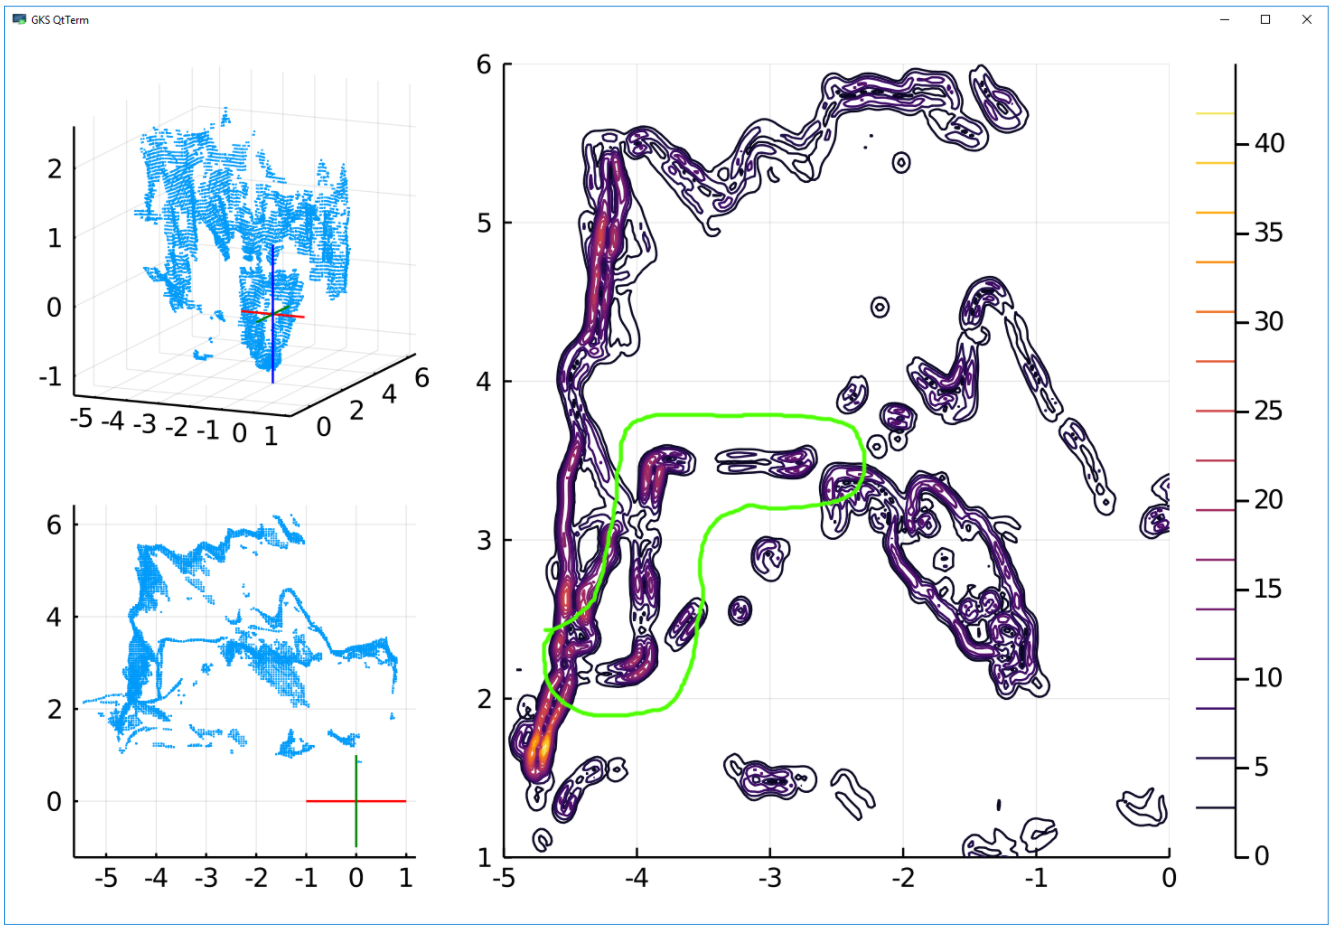
\includegraphics{mesh-to-grid-old}
